\chapter{INTRODUCTION}

{\baselineskip=2\baselineskip
	
\section{Background of the Study}

Agriculture is important in the Philippines since it serves as the foundation of food security, livelihood, and rural development. In a traditional soil management practices in the Philippines, such as those endorsed by the Department of Agriculture (DA), it relies on generalized soil health monitoring and fertilizer recommendations; they are using manual tools like the Minus-One Element Technique (MOET) and Rapid Soil Test Device (RST). These approaches often fail to address field-specific variability, crop diversity, and seasonal dynamics, leading to suboptimal resource use based on the Department of Agriculture Region 10 (2023). Historically, the method of soil testing requires transporting soil samples to the nearest laboratories located in the office of the Department of Agriculture, which was supported by the article of Pagaduan, J.L. (2025) which states that the need for farmers to transport soil samples is often expensive, time-consuming, and inaccessible in some remote places. In relation to that, the Department of Agriculture - Regional Field Office 10 (Aggie 10) conducted a soil sampling drive for soil health monitoring sites of rice and corn production areas in the towns of Sugbongcogon, Binuangan, Magsaysay and Gingoog City last March 26-28, 2025. The Aggie 10 targets to muster soil sampling and testing in priority sites across Region 10 by May 2025, in time with the wet cropping calendar based on the article from the Aggie 10 site. With the mentioned traditional method of soil testing, farmers often rely on ocular observations which was supported by the study of Samaniego, A.L. \& Gallego, M. (2024) which states that only about 1.03\% use a soil‐test kit and another 1.03\% use government lab services, while the remaining 97.94\% rely on observational methods (eyeballing the soil or plant). According to Sarma, A. et. al. (2024) crop selection decisions are frequently based on historical practices rather than data-driven insights, limiting adaptability to changing soils and climate conditions. With the use of technological advancements such as IoT it would be a great aid for the farmers to have a better crop yield and reduce loss.

The soil health is a fundamental pillar for sustainable agriculture, underpinning crop productivity, food security, and environmental resilience. According to Lal, R. (2024), degraded soils, marked by nutrient deficiencies, imbalanced pH, or reduced organic matter, lead to diminished yields, increased pest vulnerability, and economic losses for farmers. In Region 10 (Northern Mindanao, Philippines), a key agricultural hub producing rice, corn, banana, and cacao, optimal levels of nitrogen (N), phosphorus (P), potassium (K), and a pH range of 6.0–7.5 are essential for nutrient availability and robust crop growth which was mentioned on the study of Morgan \& Connolly (2013) and (Sondhiya \& Singh, 2024). According to the data from the Department of Agriculture in Region 10 last 2024, acidic soils in Bukidnon limit phosphorus uptake, while nitrogen shortages in rice fields can reduce yields by up to 20\%. Furthermore, selecting appropriate crops for specific zones and seasons, coupled with precise fertilizer application, is critical to maximizing productivity and minimizing environmental impacts like nutrient runoff (Patil et al., 2023).

Advancements in Internet of Things (IoT) technologies and machine learning (ML) offer innovative solutions for precision agriculture. IoT-based sensors, such as NPK, pH, and moisture probes, enable  soil monitoring, while ML algorithms analyze complex datasets to deliver tailored recommendations stated in the study of (Kumar et al., 2024), (Lavanya et al., 2024). Multi-Criteria Decision Analysis (MCDA) algorithms, such as Analytic Hierarchy Process (AHP) or Weighted Sum Model (WSM), further enhance decision-making by integrating multiple factors like soil nutrient profiles, climate data, and crop suitability supported by the study of Kumar \& Singh (2024). According to Elbasi et. al (2023), the modern farming methods utilizes technology to optimize crop production and minimize waste. Smart farming aids in increasing yield outputs and crop productivity. By combining IoT, ML, and MCDA with data of soil suitability maps and agricultural zoning data, systems can optimize both crop selection and fertilizer application for specific zones and seasons in Region 10.

This study proposes a Soil Health Monitoring and Recommendation System that leverages IoT sensors and a Multi-Criteria Decision Analysis (MCDA) algorithm to provide zone-specific, and season-specific recommendations for multi-cropping and fertilizer application in Region 10. Targeting key crops such as Maize (Corn), Mungbean (Mongo), Peanut, Soybean, Squash (Kalabasa), Sweet Potato (Camote), Cassava, Taro (Gabi), Eggplant, Tomato, Pechay, and Cabbage, the system integrates soil health data (NPK, pH, moisture, humidity and temperature) and agri-weather data, online data resources, and DA’s zoning maps to predict optimal crops for planting and recommend precise fertilizer strategies. By addressing field-specific variability and seasonal dynamics, the system aims to enhance agricultural productivity, reduce resource waste, and promote sustainable farming practices. Aligned with Sustainable Development Goals (SDGs) 2 (Zero Hunger), 12 (Responsible Consumption and Production), and 15 (Life on Land), this research contributes to food security, environmental conservation and goods production, and sustainable agriculture in the Philippines.


\section{Statement of the Problem}

Traditional soil management and crop selection practices in Region 10 lack precision, leading to reduced yields, resource waste, and environmental degradation (Lal. R., 20234. Generalized manual tools from Department of Agriculture tools lack accuracy to account for field-specific variability, crop diversity, and seasonal dynamics. Ultimately, the absence of data-driven fertilization recommendations and crop prediction systems limits optimal land use, particularly for Region 10’s diverse crops like Maize (Corn), Mungbean (Mongo), Peanut, Soybean, Squash (Kalabasa), Sweet Potato (Camote), Cassava, Taro (Gabi), Eggplant, Tomato, Pechay, and, Cabbage. Key challenges include:

\begin{enumerate}
	\item Ensuring accuracy of IoT sensors in monitoring soil health indicators (pH, NPK, salinity, moisture, and temperature) across farming zones in Region 10.
	\item Integration of MCDA and machine learning algorithms with soil health, climate, and zoning data to predict suitable crops and generate optimized fertilizer recommendations.
	\item Designing a mobile interface that delivers user-friendly crop and fertilizer recommendations tailored for farmers in Region 10.
	\item Evaluating the accuracy and scalability of an IoT–MCDA system in supporting agricultural practices for farmers in Region 10.
\end{enumerate}

\section{Objectives of the Study}

The main objective of this study is to develop an IoT-based crop recommender system integrated with machine learning for crop recommendation based on soil health parameters (NPK levels, pH, and moisture content) and weather data for farmers, specifically the following:

\begin{enumerate}
	\item Implement a machine learning model to predict suitable crops and recommend fertilizers for multi-cropping in Region 10 based on soil, climate, and zoning data.
	\item Develop a mobile application to monitor soil health, crop predictions, fertilizer schedules, and multi-cropping planning for farmers.
	\item Develop a website application to monitor soil health insights for different zoning, farmers data and information on their farming patterns, and multi-cropping information for each zoning.
	\item Evaluate the IoT-based crop recommender system’s accuracy and  usability in agricultural settings in Region 10.
\end{enumerate}

\section{Significance of the Study}

The significance of this study lies in its potential to transform agricultural practices in Region 10 by developing an integrated IoT and Multi-Criteria Decision Analysis (MCDA) with a machine learning model system for soil health monitoring, crop recommendation with multi-cropping, and fertilizer recommendation. Traditional methods of soil testing provided by the Department of Agriculture are not often used by farmers due to inaccessibility and time-consuming, farmers often rely on ocular observations that may involve risk in planting crops (Samaniego, A.L. \& Gallego, M., 2024). This research addresses critical limitations of traditional soil management methods, such as generalized recommendations and lack of zone-specific insights, which often lead to inefficient resource use.

By providing precise soil data and tailored crop and fertilizer suggestions for crops, the system enables farmers to optimize yields and reduce costs. Furthermore, the incorporation of DA’s zoning maps and credible online datasets enhances land use efficiency, promoting sustainable farming practices that align with environmental conservation goals. The study also contributes to precision agriculture by offering a scalable IoT-MCDA framework, facilitating data-driven decision-making for farmers. Ultimately, this research has the potential to significantly improve agricultural productivity, environmental sustainability, and food security in Region 10, supporting Sustainable Development Goals (SDGs) 2, 12, and 15.

\textbf{Farmers,} the system will greatly help the farmers in optimizing crop yield providing soil health monitoring data, and data-driven crop recommendations and optimized fertilizer use. This helps farmers to reduce risk, and maximize crop yield. 

\textbf{Department of Agriculture,} the study will aid the Department of Agriculture in Region 10 by providing real-time soil health insights, improving the accuracy of their fertilizer distribution programs, and enhancing the effectiveness of agricultural zoning. Also, it can serve as a tool for planning interventions, and monitoring soil health trends for sustainable agriculture.

\textbf{Agriculturist,} this research benefits agriculturists by serving as a reliable reference for analyzing soil conditions and crop suitability. It enhances their capacity to provide professional recommendations to farmers, reducing reliance on manual or generalized methods.

\textbf{Future Researchers,} The study will serve as a foundation for future innovations in smart farming and precision agriculture. It opens opportunities for further research in areas such as integrating remote sensing data, advanced predictive analytics, and climate-smart agriculture techniques. Future researchers can expand this system into other regions or crop categories, making it a scalable model for national and even global agricultural applications.

\section{Scope and Limitations}

This study focuses on the agricultural areas that are located in Region 10, Philippines, where specific crops such as: Maize (Corn), Mungbean (Mongo), Peanut, Soybean, Squash (Kalabasa), Sweet Potato (Camote), Cassava, Taro (Gabi), Eggplant, Tomato, Pechay, and Cabbage are produced since these crops are the focus of this study. The system was designed to analyze data input for soil health parameters such as (1) Nitrogen, (2) Phosphorus, (3) Potassium, (4) temperature,  (5) soil moisture, (6) pH level, and (7) soil salinity. These parameters are integrated with agri-weather data like leaf wetness, precipitation, temperature, and wind speed to be retrieved via a weather API that will serve as the foundation for crop recommendation and fertilizer optimization. By implementing machine learning algorithms with Multi-Criteria Decision Analysis (MCDA) methods, the system aims to promote sustainable agriculture and maximize crop yields in multi-cropping scenarios.

This study is geographically limited to farms across Bukidnon, ensuring relevant soil parameters accuracy, climate conditions, and agricultural zoning. This development emphasizes the integration of IoT, machine learning, and MCDA systems. On the other hand, the sensor that will be used for this system is limited to only seven (7) soil parameters excluding factors like micronutrients and the organic matter. Real-time soil health monitoring is not implemented, as the system focuses on periodic data analysis rather than continuous monitoring.

\subsection{Conceptual Framework}

In this section, the study’s conceptual framework is presented through an Input-Process-Output (IPO) model, which outlines the structure of the soil health monitoring, crop and fertilizer recommendation system. The framework integrates multiple components, each playing a vital role in developing an efficient, data-driven solution for sustainable agriculture.

\begin{figure}[H]
	\centering
	\caption{IPO Model}
	\label{fig:ipo}
	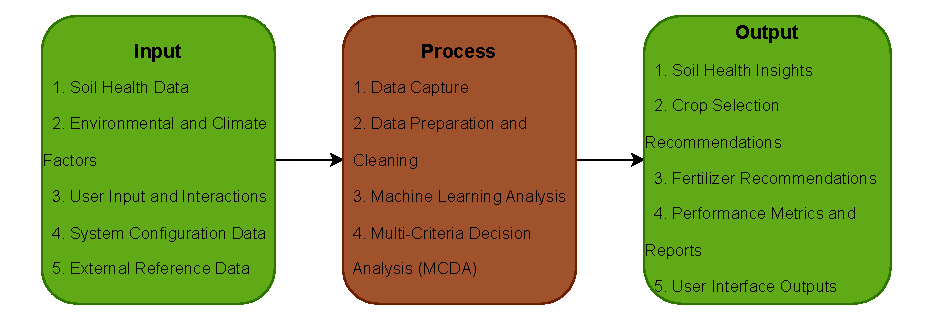
\includegraphics[width=1\textwidth]{figures/IPO.pdf}
\end{figure}

Figure 1 outlines the input, process, and output for a system designed to process soil health data and support agricultural decision-making in Region 10, Philippines. The inputs include  readings from lot sensors (NPK levels, pH, moisture, salinity, and temperature) collected via ESP32 microcontroller and Soil Sensor, zoning data from Department of Agriculture (DA) maps, historical soil data from DA Region 10 reports, environmental and climate data, online data, and farmer-defined parameters.

These inputs are then processed through data capture, cleaning, and integration with external sources, followed by machine learning analysis using LightGBM and a multi-criteria decision analysis (AHP-TOPSIS) for crop and fertilizer recommendations. The system then produces outputs such as soil health insights, zone-specific crop recommendations, fertilizer recommendations, performance metrics, and a user-friendly dashboard with  analytics, alerts, and reports. This data-driven approach enables farmers to make informed decisions, improving efficiency, yield, and resource management while reducing waste.

\subsection{Theoretical Framework}

This study utilized Precision Agriculture Theory, a strategy that gathers, processes data driven insights to optimize farming practices based on conditions rather than relying on generalized farming practices recommendations, which is supported by the study of Pierre C. Robert states that an integrated farming approach designed to enhance long-term production efficiency, productivity, and profitability while minimizing environmental impacts. It involves using technology and data to optimize farming practices at a site-specific level. The theory highlights the importance of applying the right input, at the right place, at the right time, and in the right amount to maximize productivity while conserving resources. 

With the integration of IoT sensors which will provide measurements of soil health parameters the precision agriculture theory will be fully operational. The soil parameters will serve as a foundation for the Multi-Criteria Decision Analysis methods to generate actionable recommendations for farmers. Moreover, machine learning boosting algorithms will be used to analyze soil and environmental patterns to predict crop suitability and yield potential. 

Figure 2 explains the Precision Agriculture Cycle on how farming decisions become data-driven. It starts with acquiring data through IoT sensors and other tools that measure soil and environmental conditions. This data is then processed into insights to understand soil fertility and crop needs. Using these insights, decisions are made with the help of Machine Learning (ML) for prediction and Multi-Criteria Decision Analysis (MCDA) for evaluating multiple factors like soil parameters, climate, and zoning. The next step is taking action, where farmers apply precise fertilizers, choose suitable crops, or adjust irrigation. Finally, the results and learnings feed back into the system, ensuring continuous improvement in productivity, efficiency, and sustainability.

\begin{figure}[H]
	\centering
	\caption{IPO Model}
	\label{fig:precisionagriculture}
	\includegraphics[width=0.7\textwidth]{figures/PrecisionAgriculture.pdf}
\end{figure}

By combining ML’s predictive capability with MCDA’s structured decision making process, the study applies the principles of precision agriculture in a holistic manner. This ensures that recommendations for crop selection and fertilizer application are data-driven, addressing the variability of soils and seasonal conditions in Region 10. Thus, Precision Agriculture Theory serves as the guiding lens that connects IoT-based data collection, Machine Learning prediction, and MCDA supported decision-making, ultimately promoting sustainable and efficient farming practices.

\section{Definition of Terms}

This study defined the following terms that are mentioned in this study.
	\begin{description}
	\item[Agriculture] 
	The science, art, and practice of cultivating plants and livestock, serving as the foundation for food security, livelihoods, and rural development in regions like the Philippines.
	\item[Agricultural Zoning] 
	The practice of designating specific areas for agricultural use to conserve farmland, prevent urban conflicts, and promote orderly rural growth, often including minimum lot sizes and restrictions on non-farm activities.
	\item[Analytic Hierarchy Process (AHP)] 
	A structured decision-making technique that organizes complex problems into a hierarchy of goals, criteria, and alternatives, using pairwise comparisons to derive priorities and rank options.
	\item[Boosting Algorithms] 
	A family of machine learning techniques that convert weak learners into strong ones by iteratively training models to correct errors from previous ones, commonly used in regression and classification tasks.
	\item[Crops] 
	Plants or plant products grown and harvested extensively for profit or subsistence, categorized into food, feed, fiber, oil, ornamental, and industrial types based on their uses.
	\item[Fertilizer] 
	A natural or synthetic substance added to soil to supply essential nutrients like nitrogen, phosphorus, and potassium, enhancing plant growth and productivity in agriculture.
	\item[Internet of Things (IoT) in Agriculture] 
	The integration of connected sensors, devices, and networks in farming to monitor soil, weather, crops, and livestock, enabling data-driven decisions for improved efficiency and sustainability.
	\item[Machine Learning] 
	A subset of artificial intelligence that enables computers to learn from data and improve performance on tasks without explicit programming, often using algorithms to identify patterns and make predictions.
	\item[Multi-cropping]
	The practice of growing two or more crops on the same piece of land in a single year, either sequentially or simultaneously, to enhance productivity, diversify income, and improve soil health.
	\item[Multi Criteria Decision Analysis (MCDA)]
	A decision-making approach that evaluates alternatives based on multiple conflicting criteria, using techniques like weighting and ranking to support complex choices in fields such as agriculture.
	\item[NPK]
	The abbreviation for the three primary macronutrients in soil and fertilizers: nitrogen (N), phosphorus (P), and potassium (K), essential for plant growth, development, and overall health.
	\item[Precision Agriculture]
	A farming management strategy that uses data from sensors, GPS, and analytics to optimize inputs like water and fertilizers, responding to variability in crops for improved efficiency and sustainability.
	\item[Soil Health]
	The continued capacity of soil to function as a vital living ecosystem that sustains plants, animals, and humans, encompassing biological, physical, and chemical properties.
	\item[Soil pH]
	A measure of soil acidity or alkalinity on a scale from 0 to 14, indicating hydrogen ion concentration, which influences nutrient availability and plant growth.
	\item[Soil Salinity]
	The accumulation of soluble salts in soil that can impair plant growth, often measured by electrical conductivity, with levels above 4 dS/m considered saline.
	\item[Sustainable Agriculture]
	Farming practices that meet current food needs while preserving resources for future generations, balancing environmental health, economic viability, and social equity.
	
	\end{description}
}